\subsection{Newton’s Fluxions: Motion and Tangents}  

Newton approached calculus as an extension of physical motion, and grounded it in the geometric traditions of antiquity. Inspired by thinkers like Euclid, who formalized the structure of geometry, and Pythagoras, who explored the relationships between lengths and proportions, Newton developed his system of calculus through the lens of space, motion, and change.

But Newton didn’t just imitate classical methods—he expanded them. Euclid, for instance, assumed that a tangent line could be drawn to a circle and proved its properties using geometric reasoning. However, he did not offer a general method for constructing tangents to arbitrary curves. Newton changed that.

With his concept of \textit{fluxions}, Newton introduced a systematic way to find the instantaneous rate of change of a quantity—effectively, to construct a tangent not just to a circle, but to *any* curve. Where Euclid began with tangents as given, Newton derived them from first principles of motion. The tangent became not a geometric assumption, but the result of a dynamic process.

This shift—from static geometry to the mathematics of continuous change—marked a foundational leap. Newton’s fluxions allowed him to describe motion, curvature, and accumulation with unprecedented precision.

\[
\dot{x} = \frac{o}{\bar{o}}
\]

where:  
\begin{itemize}
    \item \( o \) is an \textbf{infinitely small increment} of time.  
    \item \( \bar{o} \) is the corresponding change in \( x \).  
\end{itemize}  

\begin{figure}[H]
\centering
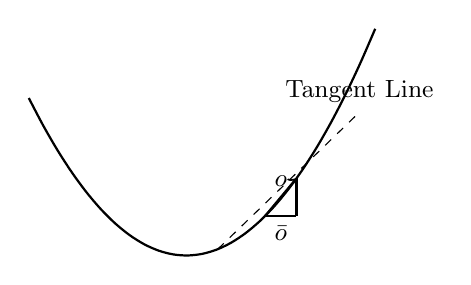
\begin{tikzpicture}[scale=2]
    % Draw the curve
    \draw[thick, domain=-1:1.2, smooth, variable=\x] plot ({\x},{\x*\x});

    % Draw infinitesimal motion
    \draw[->, thick] (0.5, 0.25) -- (0.7, 0.49) node[midway, above] {\small $o$};
    \draw[thick] (0.5, 0.25) -- (0.7, 0.25);
    \draw[thick] (0.7, 0.25) -- (0.7, 0.49);
    \node[below] at (0.6,0.25) {\small $\bar{o}$};
    
    % Draw tangent line
    \draw[dashed] (0.2, 0.04) -- (1.1, 0.91) node[above] {\small Tangent Line};

\end{tikzpicture}

\vspace{0.5em}
\caption{\small Newton's conception of calculus was rooted in geometry and motion. He imagined a point moving along a curve, where the instantaneous rate of change — the fluxion — could be represented as the ratio between an infinitesimal vertical change ($o$) and an infinitesimal horizontal change ($\bar{o}$). The resulting quantity corresponds to the slope of the tangent line at that point. This approach reflects Newton’s view of change as inherently tied to physical movement through time.}
\end{figure}


For Newton, the fluxion — or derivative — was the geometric expression of velocity: a quantity changing over time. His thinking preserved the visual and spatial intuition of Euclid and Pythagoras, using infinitesimal right triangles to model continuous motion and instantaneous change.
